Having established and validated the tools for the quantification of bovine \textit{IFITs}, as well as elucitaded the optimal assay termination time points for bRSV infections we then had all the tools required to mirror the analysis from Chapter \ref{ch:Assessment of Transcriptional Induction of Human IFITs in the Context of RSV}. That is, we wnated to systematically assay the \textit{bIFIT} induction, firstly by using different activators of innate immune system, following by bRSV infection and lastly assessing the cross-species defence by hRSV infection. The relative induction levels would be assayed using RT-qPCR methodology as described in Section \ref{sec:Quantitative Real Time/Reverse Transcription PCR}. Briefly, cells were cultivated in 12-well plates and subsequently exposed to the respective stimulants. At the endpoint of the experiments, RNA extraction was performed, followed by complementary DNA (cDNA) synthesis and transcript quantification through qPCR. \textit{hRSV N}, \textit{bRSV N}, and \textit{bMx1} genes were quantified using the \(\Delta\)\(\Delta\)Ct method, normalised to bovine \textit{GAPDH} gene, and subsequently further normalized against mock-treated samples. As described previously, bovine \textit{IFIT} genes copy numbers were extrapolated from standard curves, freshly created per experiment, normalised relative to the mock copy numbers and further factorised to the relative levels of bovine \textit{GAPDH} detected per experimental conditions. The statistical analysis adhered to the procedures outlined in Section \ref{sec:Statistical Analysis}. It is important to note that the selection of the appropriate statistical test was contingent upon the assessment of data distribution normality and the equality of variance, considerations that will be elaborated upon in the subsequent sections of this chapter.

\subsection{Bovine \textit{IFIT} Responses to Activators of Innate Immune Response} \label{subsec:Bovine IFIT Responses to Activators of Innate Immune Response}
The Madin-Darby bovine kidney (MDBK) cell line, derived from bovine renal epithelium in 1958 (\cite{Madin1958EstablishedOrigin}), is a well-established model system used in bovine virology studies. We assayed the cells for the induction potential of bovine \textit{IFITs}, alongside bovine \textit{Mx1} using bovine interferon alpha and LPS (bovine interferon-gamma was not available commercially). Bovine \textit{Mx1} was included in the analyses as it is a ISG, widely reported in immunology and virology studies (ADD SOME REFERENCES HERE FOR CRYING OUT LOUD), and because we saw minimal bovine \textit{IFIT} responses throughout the study and wanted to ensure the cell lines used had the internal pathways for ISG induction correctly functioning. Figure \ref{fig:MDBK responses to bIFNa} shows the \textit{bIFIT} and \textit{bMx1} responses to the stimulation with bIFN\(\alpha\) at a concentration of 5 ng/mL (equivalent to 1,000 UI/mL of hIFN\(\alpha\)) for either 3 or 6 hours.

We can see that all assayed genes get biologically significantly upregulated by 3 hours of induction, althought the magnitude varies substantially. In terms of bovine \textit{IFITs}, all display higher induction at 3 hours compared to 6 hours. The \textit{bIFITs} exhibit similar patter of induction to what was observed with A549, that is \textit{bIFIT1} exhibitng the strongest response, while \textit{bIFIT2} and \textit{bIFIT3} showing medium responses of similar amplitudes, and finally \textit{bIFIT5} exhibiting the lowest responses. \textit{bIFIT1} shows the highest induction at 20-fold and 5-fold respectively and is the only bovine \textit{IFIT} that exhibits biologically significant induction at 6 hours of incubation. \textit{bIFIT2} and \textit{bIFIT3} were induced by 6-fol and 3.5-fold for 3 hour and 6 hour incubation with bIFN\(\alpha\) respectivelly. \textit{bIFIT5} was induced by 4-fol and 2-fold respectively. With regards to \textit{bMx1}, we can see its response to superseeds the ones of bovine \textit{IFITs}, while the patter of induction is changed as well. We see time dependant induction that increases from 32-fold to 120-fold as the treatment continues. This shows that MDBK cells are capable of \textit{bIFIT} and \textit{bMx1} induction, although with differential temporal dynamics, however, the responses are modest, especially comared to the previously obseved human \textit{IFIT} responses to IFN\(\alpha\). As a side note, while \textit{bIFIT3} and \textit{bIFIT5} datasets exhibited normal distribution of data with equal variances, \textit{bIFIT1}, \textit{bIFIT2}, and \textit{bMx1} datasets exhibited normal distributions with unequal variances.

\begin{figure}
    \centering
    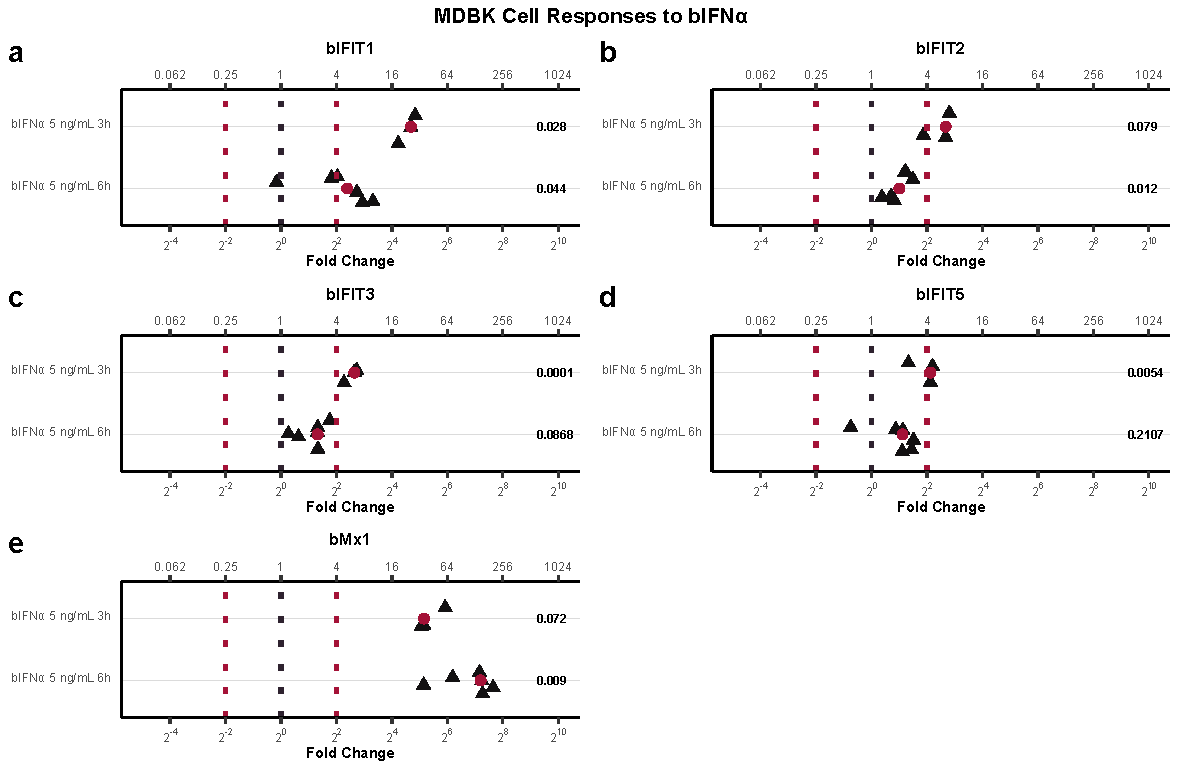
\includegraphics[width=1\linewidth]{07. Chapter 2/Figs/02. Induction/01. mdbk_treat_bifna.pdf}
    \caption[\textit{bIFIT} Gene Expression in MDBK Cells in Response to bIFN\(\alpha\) Stimulation.]{\textbf{\textit{bIFIT} Gene Expression in MDBK Cells in Response to bIFN\(\alpha\) Stimulation.} (a) \textit{bIFIT1}, (b) \textit{bIFIT2}, (c) \textit{bIFIT3}, (d) \textit{bIFIT5}, and (e) \textit{bMx1} gene expression levels were assessed using quantitative real-time PCR (qPCR) in MDBK cells following stimulation with bovine interferon alpha (IFN\(\alpha\)) at a concentration of 5 ng/mL for a treatment duration of either 3 or 6 hours. Relative expression values are normalized to standardized mock-treated samples. Median values are represented by red circles. The black dotted line represents mock expression levels, while the red dotted lines indicate biologically significant induction thresholds. Numeric values indicate the p-values compared to mock-treated samples.}
    \label{fig:MDBK responses to bIFNa}
\end{figure}

Furthermore, we wanted to investigate the invovement of Toll-like Receptor 4 (TLR4) in bovine \textit{bIFIT} induction, as we previously oberved it to be involved in A549 cell line (Figure \ref{fig:A549 Response to LPS} from Section \ref{subsec:Human IFIT Responses to Activators of Innate Immune Response}). We incubated the MDBK cells with LPS for 6 hours at concentrations of 0.5, 1, 2.5, 5, and 10 ng/mL. Aftwerwards, the cells were lysed and their RNA extracted, converted to cDNA and quantified by qPCR as described previously. We can see that neither \textit{bMx1} nor \textit{bIFITs} are induced to biologically significant levels by LPS in the concentration range tested. While most time points yield no relative change, 2.5 ng/mL cause \textit{bIFIT1}, \textit{bIFIT2}, and \textit{bIFIT3} levels to drop by half. Clearly the data suggest that LPS at the concentrations tested does not induce neither \textit{bMx1} nor \textit{bIFITs}, and if anything causes a slight downregulation of their expression. As a side note, while \textit{bIFIT3}, \textit{bIFIT5}, and \textit{bMx1} datasets exhibited normal distribution of data with equal variances, \textit{bIFIT1} and \textit{bIFIT2} datasets exhibited normal distributions with unequal variances.


\begin{figure}
    \centering
    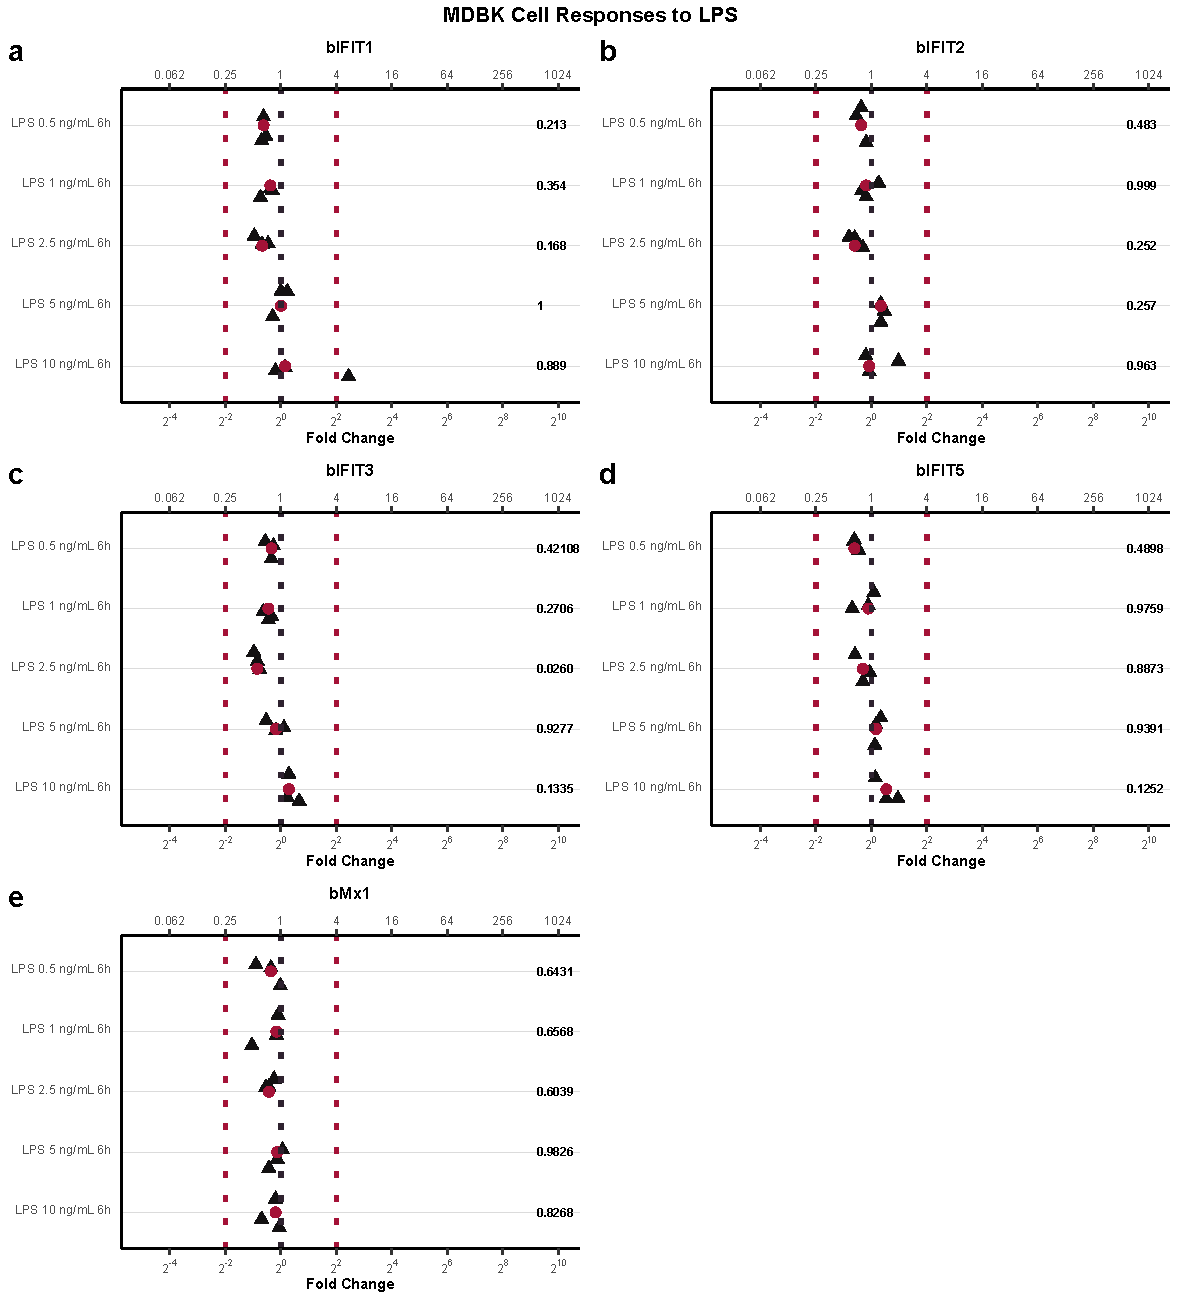
\includegraphics[width=1\linewidth]{07. Chapter 2/Figs/02. Induction/02. mdbk_treat_lps.pdf}
    \caption[\textit{bIFIT} Gene Expression in MDBK Cells in Response to LPS Stimulation.]{\textbf{\textit{bIFIT} Gene Expression in MDBK Cells in Response to LPS Stimulation.} (a) \textit{bIFIT1}, (b) \textit{bIFIT2}, (c) \textit{bIFIT3}, (d) \textit{bIFIT5}, and (e) \textit{bMx1} gene expression levels were assessed using quantitative real-time PCR (qPCR) in MDBK cells following stimulation with bacterial LPS at a concentration of 0.5, 1, 2.5, 5, and 10 ng/mL for a treatment duration of 6 hours. Relative expression values are normalized to standardized mock-treated samples. Median values are represented by red circles. The black dotted line represents mock expression levels, while the red dotted lines indicate biologically significant induction thresholds. Numeric values indicate the p-values compared to mock-treated samples.}
    \label{fig:MDBK responses to LPS}
\end{figure}

To validate the MDBK induction data we used BT cell line. It originates in a Bovine viral diarrhea virus (BVDV) negative bovine nasal turbinate cells, isolated in 1974 from neonatal Holstein cow (\cite{McClurkin1974ComparisonVirus}). As described in Section \ref{Growth Curves of Bovine RSV in Bovine Cell Lines}, these cells enable bRSV replication while originates from more physiologically significant place for bRSV life cycle than MDBK cell line. We incubated the BT cells with 5 ng/mL of bIFN\(\alpha\) for the duration of either 3 hours or 24 hours. Figure \ref{fig:BT responses to bifna} shows the results. We can see that while at 3 hours of treatment all genes but \textit{bIFIT2} are induced to biologically significant levels, after 24 hours the relative mRNA levels return to basal levels. In more detail, \textit{bIFIT1} is the highest responder with 20-fold innduction, followed by \textit{bMx1}, with 16-fold increase. \textit{bIFIT3} is induced 8-fold, while \textit{bIFIT5} 4-fold. As a side note, while \textit{bIFIT2} dataset exhibited normal distribution of data with equal variances, all other datasets exhibited normal distributions with unequal variances. All together, we can conclude that the BT cell line is interferon sensitive and \textit{bIFIT} induction competent. This data also agrees with the MDBK data (from Figure \ref{fig:MDBK responses to bIFNa}), where the \textit{bIFITs} respond acutely to bIFN\(\alpha\) stimulation, although the induction is not persistent by 24 hours. The differences are lost of induction persistance of \textit{bMx1} and lack of bIFN\(\alpha\) sensitivity by \textit{bIFIT2}.

\begin{figure}
    \centering
    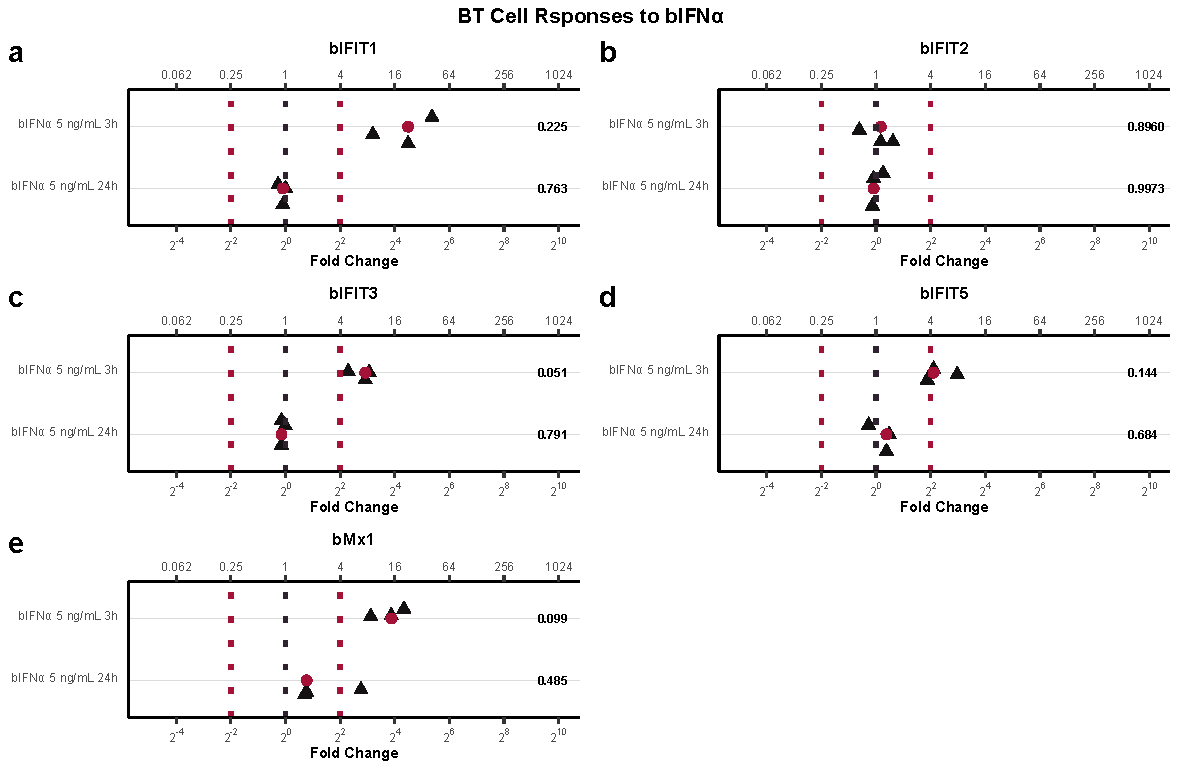
\includegraphics[width=1\linewidth]{07. Chapter 2/Figs/02. Induction/08. bt_bifna.pdf}
    \caption[\textit{bIFIT} Gene Expression in BT Cells in Response to bIFN\(\alpha\) Stimulation.]{\textbf{\textit{bIFIT} Gene Expression in BT Cells in Response to bIFN\(\alpha\) Stimulation.} (a) \textit{bIFIT1}, (b) \textit{bIFIT2}, (c) \textit{bIFIT3}, (d) \textit{bIFIT5}, and (e) \textit{bMx1} gene expression levels were assessed using quantitative real-time PCR (qPCR) in BT cells following stimulation with bovine interferon alpha (IFN\(\alpha\)) at a concentration of 5 ng/mL for a treatment duration of either 3 or 24 hours. Relative expression values are normalized to standardized mock-treated samples. Median values are represented by red circles. The black dotted line represents mock expression levels, while the red dotted lines indicate biologically significant induction thresholds. Numeric values indicate the p-values compared to mock-treated samples.}
    \label{fig:BT responses to bifna}
\end{figure}

\subsection{Bovine \textit{IFITs} Responses to bRSV} \label{subsec:Bovine IFITs Responses to bRSV}
Confirming that the cell lines selected are \textit{bIFIT} induction competent, we wanted to assess the effect of bRSV infection on \textit{bIFIT} induction, especially the effect of varying viral MOI and the duration of infection. To do this, we infected the MDBK cells with crude extracted bRSV at MOIs of 0.1, 1, and 2 for duration of 24 and 48 HPI. The virus used in these experiments was prepared and quantified as outlined in Section \ref{subsec:Virus Propagation and Production} and Section \ref{subsec:Virus Quantification by TCID50 Assay}. 

\begin{figure}
    \centering
    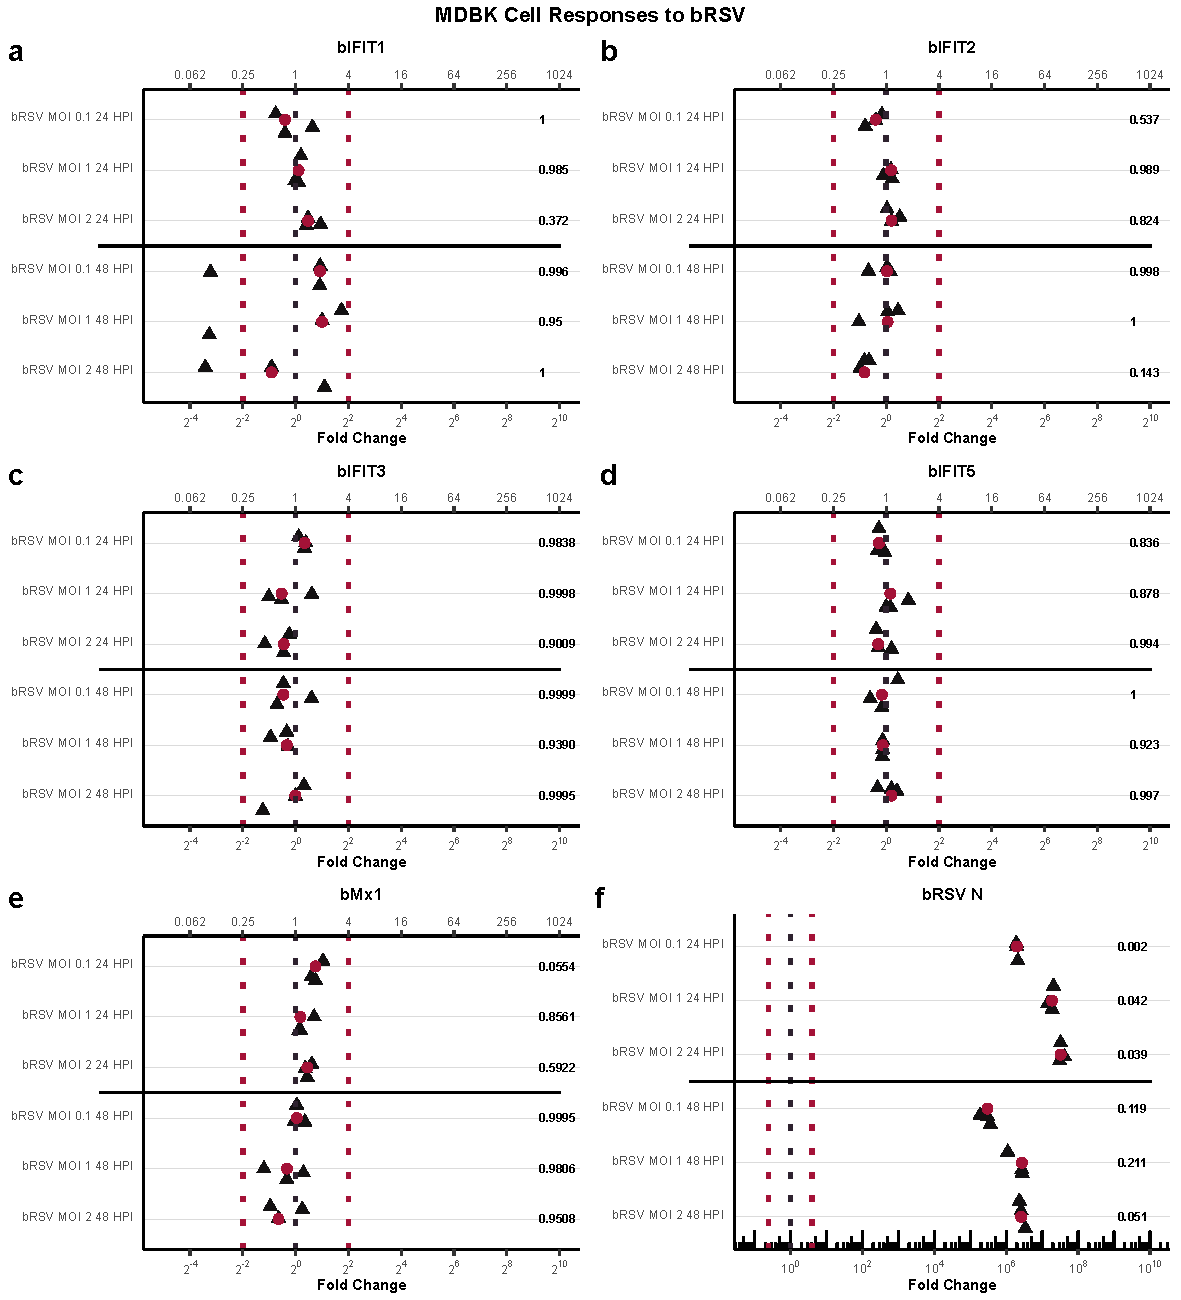
\includegraphics[width=1\linewidth]{07. Chapter 2/Figs/02. Induction/03. mdbk_brsv_timepoints.pdf}
    \caption[MDBK \textit{bIFIT} Response to bRSV Infection as a Function of Time and MOI.]{\textbf{MDBK \textit{bIFIT} Response to bRSV Infection as a Function of Time and MOI.} (a) \textit{bIFIT1}, (b) \textit{bIFIT2}, (c) \textit{bIFIT3}, (d) \textit{bIFIT5}, (e) \textit{bMx1} and (f) \textit{bRSV N} gene expression levels were assessed using quantitative real-time PCR (qPCR) in MDBK cell line following infection with bovine RSV at MOI of either 0.1, 1, or 2 for either 24 or 48 hours post-infection. Relative expression values are normalized to standardized mock-treated samples. Median values are represented by red circles. The black dotted line represents mock expression levels, while the red dotted lines indicate biologically significant induction thresholds. Numeric values indicate the p-values compared to mock-treated samples.}
    \label{fig:MDBK responses to bRSV timepoints}
\end{figure}

Figure \ref{fig:MDBK responses to bRSV timepoints} shows the results of this experiment. We can see that while the bRSV was successfully replicating, as is highlighted by the high relative \textit{bRSV N} values for all MOIs and HPIs tested (panel f), neither \textit{bMx1} nor \textit{bIFITs} show biologically significant alteration of mRNA levels. While \textit{bIFIT3}  and \textit{bIFIT5} mRNA levels stayed unchanged for all conditions, we see small positive and negative changes for the other genes. \textit{bIFIT1} levels doubled for infections with 0.1 and 1 MOI 48 HPI, and decreased by half at MOI 2 48 HPI. \textit{bIFIT2} mRNA levels were unchanged other than in 2 MOI infection at 48 HPI. \textit{bMx1} was induced 2-fold by 0.1 MOI infection, 24 HPI and downregulated by half after 2 MOI infection 48 HPI. From the statistical point of view, the datasets of \textit{bIFIT3} and \textit{bMx1} showed normal distributions and equal variences, while the other were of normal distribution with unequal variances. It is interesting to see minimal responses to bRSV infection, especially as our human data from Chapter \ref{ch:Assessment of Transcriptional Induction of Human IFITs in the Context of RSV} suggest that the \textit{hIFIT} responses are mainly mediated by the action of interferon alpha and from Section \ref{subsec:Bovine IFIT Responses to Activators of Innate Immune Response} we know that \textit{bIFITs} and especially \textit{bMx1} respond to bovine interferon alpha stimulation. It is probable that some bRSV constituents, or certain cytokines or chemocines in the crudly extracted bRSV preparations are inhibiting the cascades that would allow for \textit{bIFIT} induction.

\begin{figure}
    \centering
    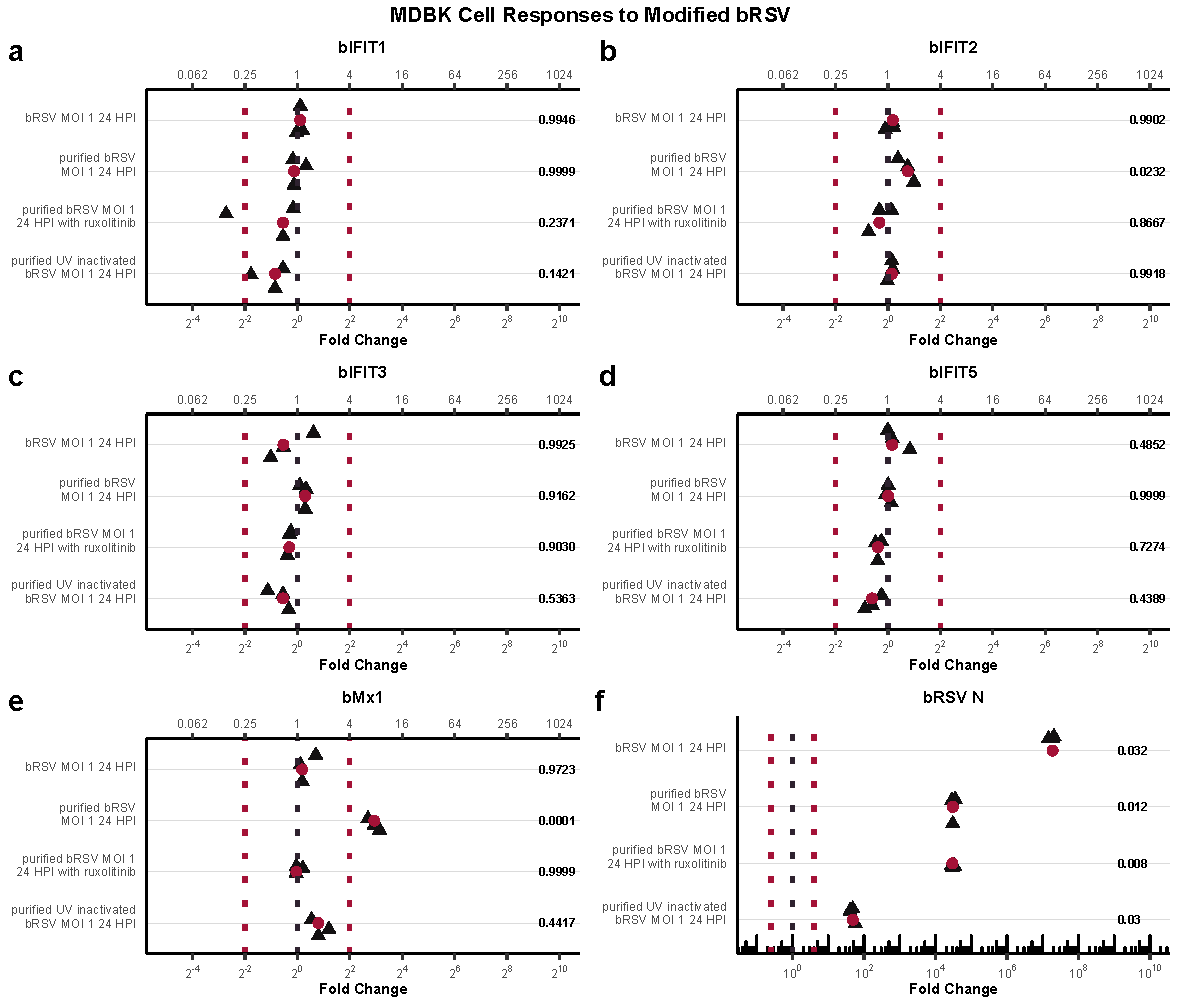
\includegraphics[width=1\linewidth]{07. Chapter 2/Figs/02. Induction/04. mdbk_brsv_uv_roxo.pdf}
    \caption[Impact of Ultra-Purification, UV-Inactivation, and INFR Inhibition on \textit{bIFIT} Induction in MDBK Cells Following bRSV Infection.]{\textbf{Impact of Ultra-Purification, UV-Inactivation, and INFR Inhibition on \textit{bIFIT} Induction in MDBK Cells Following bRSV Infection.} (a) \textit{bIFIT1}, (b) \textit{bIFIT2}, (c) \textit{bIFIT3}, (d) \textit{bIFIT5}, (e) \textit{bMx1}, and (f) \textit{bRSV N} gene expression levels were assessed using quantitative real-time PCR (qPCR) in MDBK cell line following infection with ultra-purified bRSV at MOI 1 for 24 hours. The cells were subjected to three different conditions: virus infection alone (top row), virus infection in the presence of 5 nM of ruxolitinib (interferon receptor inhibitor) throughout the infection (middle row), or UV-inactivated bRSV infection (bottom row). Relative expression values are normalized to standardized mock-treated samples. Median values are represented by red circles. The black dotted line represents mock expression levels, while the red dotted lines indicate biologically significant induction thresholds. Numeric values indicate the p-values compared to mock-treated samples.}
    \label{fig:The effect of ultra-purification, UV-inactivation and INFR inhibition on hIFIT induction following hRSV infection in MDBK}
\end{figure}

To investigate the latter, we infected the MDBK cells with ultrapurified bRSV, prepared by ultra-centrifugation on a discontinuous sucrose cushion, as described in Section \ref{subsec:Virus Propagation and Production}. Along to this, we wanted to assess the effect of pharmacological inhibition of interferon receptor and physical bRSV inactivation on \textit{bIFIT} and \textit{bMx1} induction. We did this as we previously decribed in Section \ref{subsec:Human IFITs Responses to Human RSV}, Figure \ref{fig:The effect of ultra-purification, UV-inactivation and INFR inhibition on hIFIT induction following hRSV infection in BEAS-2B} how basal interferon receptor activation is required for the maintainance of basal \textit{hIFIT} mRNA expression. The data can be observed in Figure \ref{fig:The effect of ultra-purification, UV-inactivation and INFR inhibition on hIFIT induction following hRSV infection in MDBK}. We can see that the viral purification status did not influence the induction of \textit{bIFITs}, however, ultra-purification caused a 7-fold induction of \textit{bMx1}. This was reversed completely by the presence of interferon receptor inhibitor, ruxolitinib. Its presence also slightly decreased the abundance of all \textit{bIFIT} mRNA, although not to a biologically significant levels. Interestingly, the relative median \textit{bRSV N} mRNA value was maintained between the first two conditions. This is in contrast to what we observed in human samples where the presence of ruxolitinib increased the relative median \textit{bRSV N} mRNA. Lastly, we can see that UV-inactivation of bRSV caused only small changes for all genes of magnitude of circa \(\pm\)2. Taken together, we can see that \textit{bMx1} induction response mirrors to what was observed with human RSV in A549 and BEAS2B cell lines in Chapter \ref{ch:Assessment of Transcriptional Induction of Human IFITs in the Context of RSV}. On the other hand, we did not see any significant alterations of \textit{bIFIT} mRNA levels. This suggest that some cellular contaminant present in crude extracted bRSV preparations were suppressing the induction of \textit{bMx1}, but their absence was irrelevant to the potential \textit{bIFIT} induction inhibition. As a side note, while \textit{bIFIT3} and \textit{bMx1} datasets exhibited normal distribution of data with unequal variances, \textit{bIFIT1}, \textit{bIFIT2}, \textit{bIFIT3}, and \textit{bIFIT5} datasets exhibited normal distributions with equal variances.

\begin{figure}
    \centering
    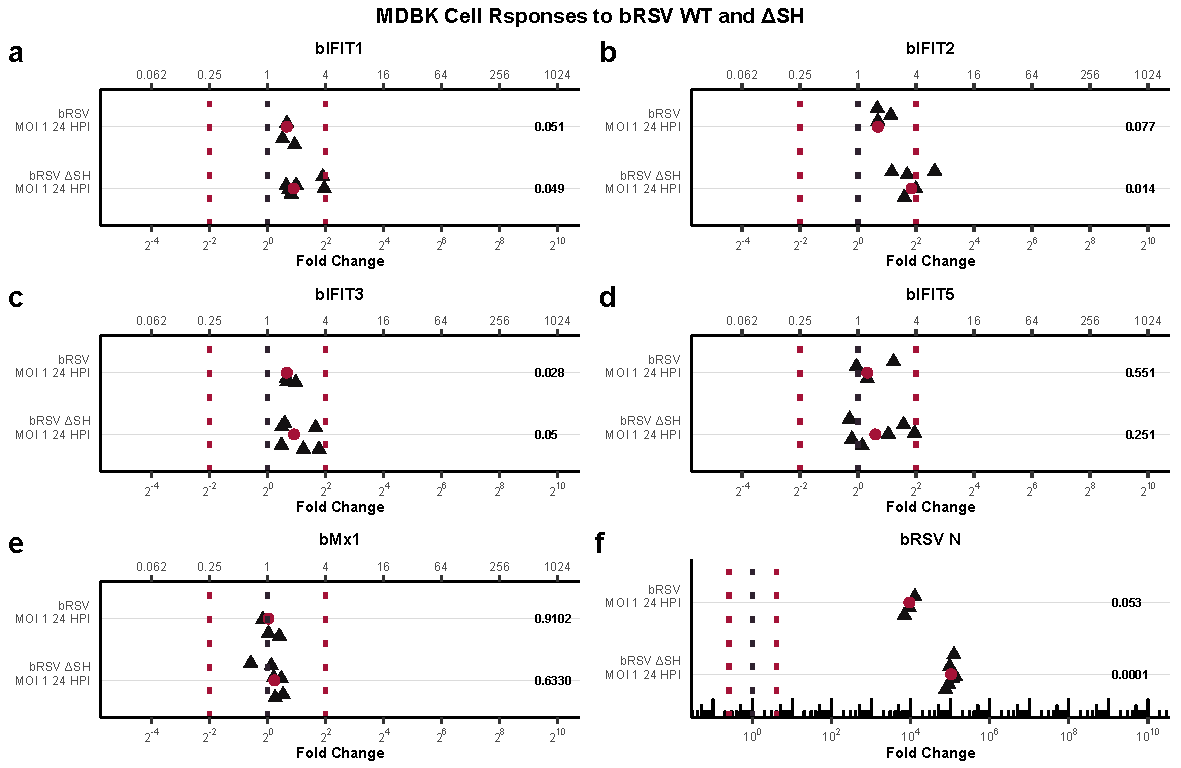
\includegraphics[width=1\linewidth]{07. Chapter 2/Figs/02. Induction/05. mdbk_brsv_moi1_dsh.pdf}
    \caption[MDBK \textit{bIFIT} Response to WT and \(\Delta\)SH bRSV Infection.]{\textbf{MDBK \textit{bIFIT} Response to WT and \(\Delta\)SH bRSV Infection.} (a) \textit{bIFIT1}, (b) \textit{bIFIT2}, (c) \textit{bIFIT3}, (d) \textit{bIFIT5}, (e) \textit{bMx1}, and (f) \textit{bRSV N} gene expression levels were assessed using quantitative real-time PCR (qPCR) in MDBK cell line following infection with WT or \(\Delta\)SH bRSV at MOI 1 for 24 hours post-infection. Relative expression values are normalized to standardized mock-treated samples. Median values are represented by red circles. The black dotted line represents mock expression levels, while the red dotted lines indicate biologically significant induction thresholds. Numeric values indicate the p-values compared to mock-treated samples.}
    \label{fig:MDBK responses to dSH}
\end{figure}



mdbk dsh

wt bRSV along with MOI 1 dSH do not up or downregulate any genes tested in a biologically significant way.

normal unequal - bi1 bi2 bi3 bi5 brsvn

normal euqal - bmx1

%brsvn 10^4 10^5
%    10^3 10^5 on a549 and beas2b
%    mdbk puri 10^4.5 10^7.2

2 sig @ 4 dSH
3 mx1 nothing
something in crude extracts inhubits induction?


\begin{figure}
    \centering
    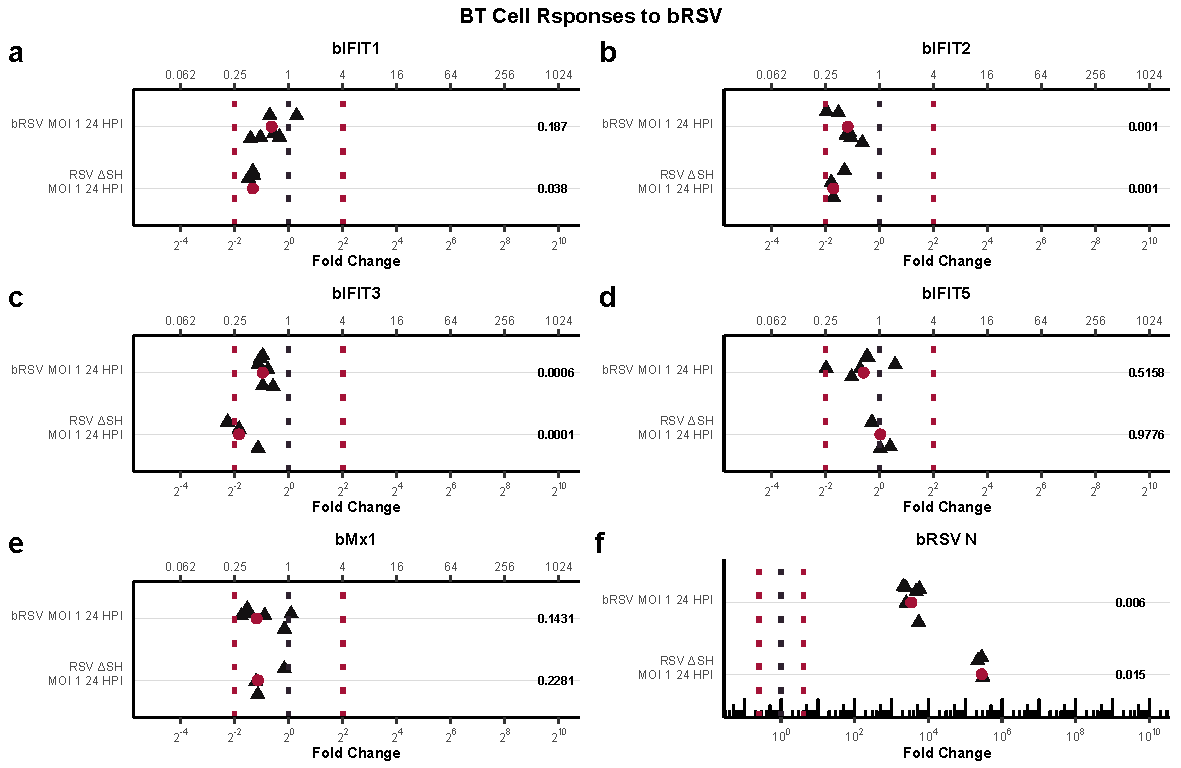
\includegraphics[width=1\linewidth]{07. Chapter 2/Figs/02. Induction/09. bt_brsv.pdf}
    \caption[BT \textit{bIFIT} Response to WT and \(\Delta\)SH bRSV Infection.]{\textbf{BT \textit{bIFIT} Response to WT and \(\Delta\)SH bRSV Infection.} (a) \textit{bIFIT1}, (b) \textit{bIFIT2}, (c) \textit{bIFIT3}, (d) \textit{bIFIT5}, (e) \textit{bMx1}, and (f) \textit{bRSV N} gene expression levels were assessed using quantitative real-time PCR (qPCR) in BT cell line following infection with WT or \(\Delta\)SH bRSV at MOI 1 for 24 hours post-infection. Relative expression values are normalized to standardized mock-treated samples. Median values are represented by red circles. The black dotted line represents mock expression levels, while the red dotted lines indicate biologically significant induction thresholds. Numeric values indicate the p-values compared to mock-treated samples.}
    \label{fig:BT responses to bRSV}
\end{figure}

bt dsh and wt brsv

Infections with wt bRSV and dSH bRSV at the same MOI and HPI (1 and 24) cause slight downregulation in all genes tested.

normal unequal - bi1 brsvn

normal euqal - bi2 bi3 bi5 bmx1

%brsvn 10^3.3 10^5.2
decrease in most
2 and 3 the same
1/2 and sig 1/4
mx1 both same just below 1/2
1 same profile as 2 3 
    just above 1/2 1/4
5 wt same as 1, dSH nothing


\begin{figure}
    \centering
    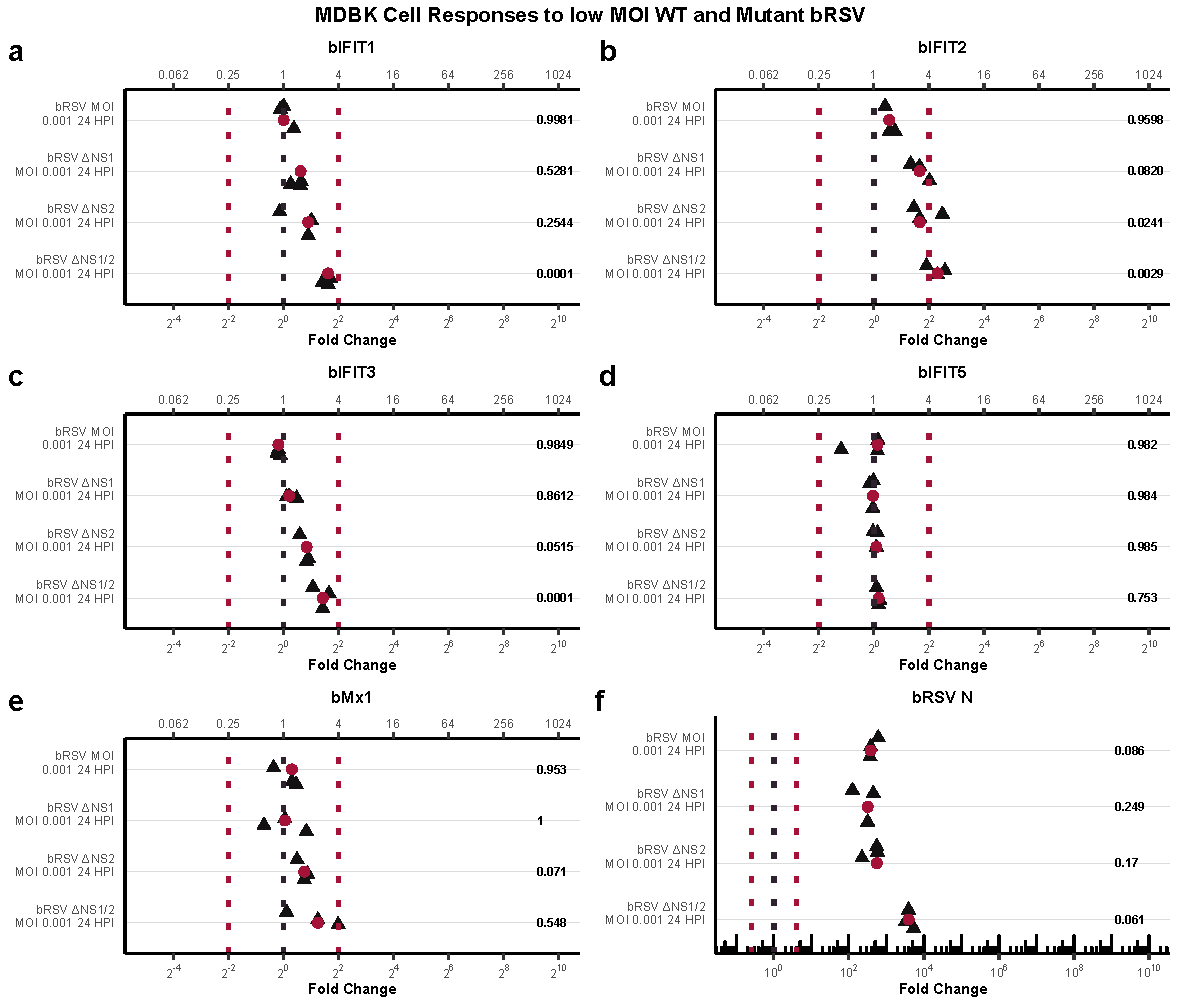
\includegraphics[width=1\linewidth]{07. Chapter 2/Figs/02. Induction/06. mdbk_brsv_low_moi.pdf}
    \caption[MDBK \textit{bIFIT} Response to Low MOI bRSV Infections.]{\textbf{MDBK \textit{bIFIT} Response to Low MOI bRSV Infections.} (a) \textit{bIFIT1}, (b) \textit{bIFIT2}, (c) \textit{bIFIT3}, (d) \textit{bIFIT5}, (e) \textit{bMx1}, and (f) \textit{bRSV N} gene expression levels were assessed using quantitative real-time PCR (qPCR) in MDBK cell line following infection with WT or \(\Delta\)NS1, \(\Delta\)NS2, and \(\Delta\)NS1/2 bRSV at MOIs of 0.001 for 24 hours post-infection. Relative expression values are normalized to standardized mock-treated samples. Median values are represented by red circles. The black dotted line represents mock expression levels, while the red dotted lines indicate biologically significant induction thresholds. Numeric values indicate the p-values compared to mock-treated samples.}
    \label{fig:MDBK responses to low MOI mutant bRSV}
\end{figure}

low moi dnss mdbk

Very low MOI (0.001) wt bRSV along with MOI 1 dSH and very low MOI dNS1, dSN2 and dNS1/2 bRSV do not up or downregulate any genes tested in a biologically significant way.

normal unequal - bi5 bmx1 brsvn

normal euqal - bi1 bi2 bi3 

%brsvn 10^3.5 10^3.3 10^3.6 10^4.4
5 nothing for all
1 3 the same    1 1.5 2 3.4
2 -> 1.5 3.5 3.5 4
bmx1 -> 1 1 2 3

completely different to a549
    also diff moi



\subsection{Bovine \textit{IFITs} Responses to hRSV} \label{subsec:Bovine IFITs Responses to hRSV}

Intro into hrsv infections


\begin{figure}
    \centering
    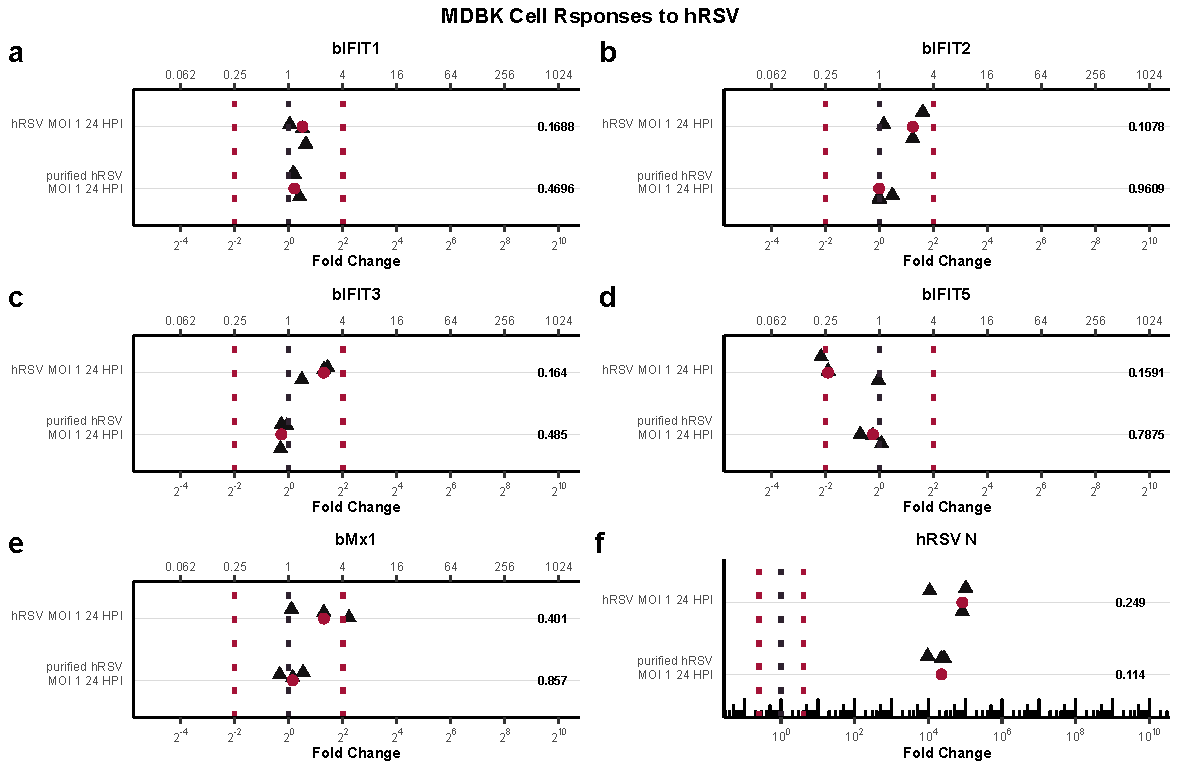
\includegraphics[width=1\linewidth]{07. Chapter 2/Figs/02. Induction/07. mdbk_hrsv.pdf}
    \caption[MDBK \textit{bIFIT} Response to Crude-Extracted and Ultra-Purified hRSV Infection.]{\textbf{MDBK \textit{bIFIT} Response to Crude-Extracted and Ultra-Purified hRSV Infection.} (a) \textit{bIFIT1}, (b) \textit{bIFIT2}, (c) \textit{bIFIT3}, (d) \textit{bIFIT5}, (e) \textit{bMx1}, and (f) \textit{hRSV N} gene expression levels were assessed using quantitative real-time PCR (qPCR) in MDBK cell line following infection with crude-extraccted and ultra-purified hRSV at MOI 1 for 24 hours post-infection. Relative expression values are normalized to standardized mock-treated samples. Median values are represented by red circles. The black dotted line represents mock expression levels, while the red dotted lines indicate biologically significant induction thresholds. Numeric values indicate the p-values compared to mock-treated samples.}
    \label{fig:bIFIT responses to hRSV infection in MDBK}
\end{figure}

mdbk hrsv

Data show that ultracentrifugation purified hRSV causes no response in terms of bIFIT induction. Infection with normally purified virus does not cause induction either but hints at downregulation actually.

normal unequal - bi5 bmx1 brsvn

normal euqal - bi1 bi2 bi3 

%hrsv n 10^5 10^4.2
0 response to puri for all
2 3 bmx1 same response to crude @ 3
1 small increase crude @ 1.5
5 sig down crude 1/4


\begin{figure}
    \centering
    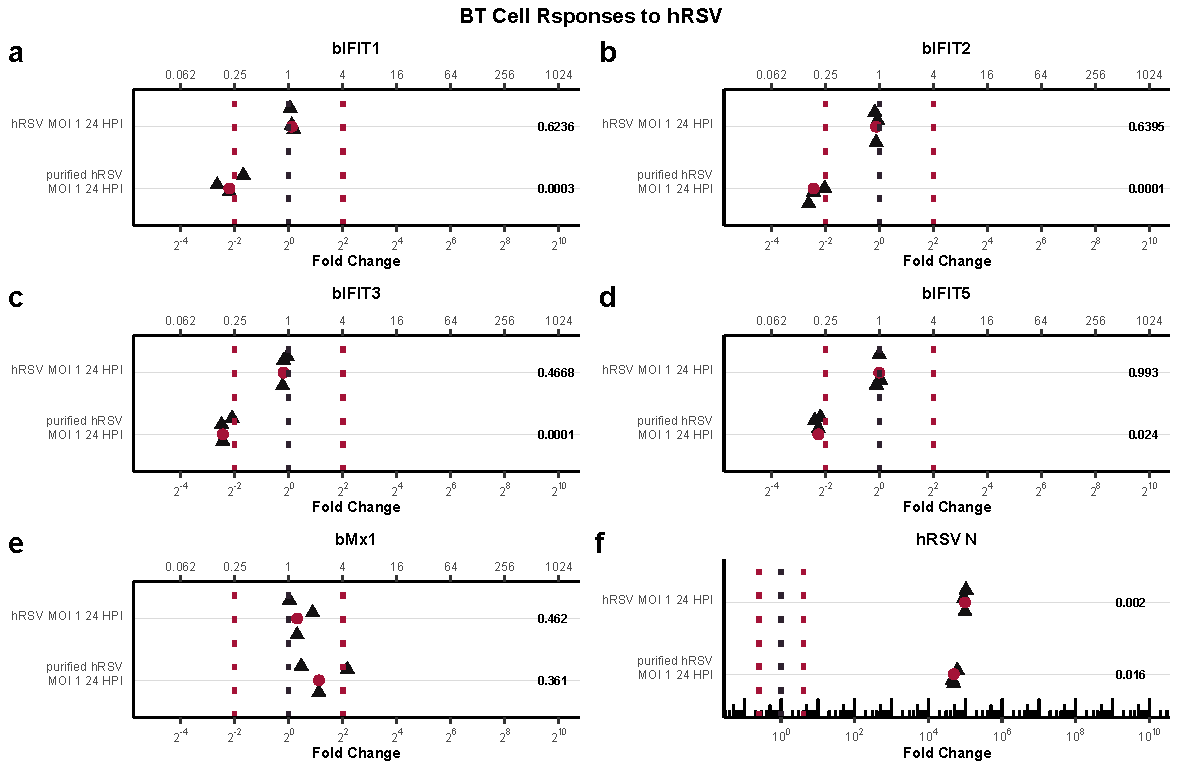
\includegraphics[width=1\linewidth]{07. Chapter 2/Figs/02. Induction/10. bt_hrsv.pdf}
    \caption[BT \textit{bIFIT} Response to Crude-Extracted and Ultra-Purified hRSV Infection.]{\textbf{BT \textit{bIFIT} Response to Crude-Extracted and Ultra-Purified hRSV Infection.} (a) \textit{bIFIT1}, (b) \textit{bIFIT2}, (c) \textit{bIFIT3}, (d) \textit{bIFIT5}, (e) \textit{bMx1}, and (f) \textit{hRSV N} gene expression levels were assessed using quantitative real-time PCR (qPCR) in BT cell line following infection with crude-extraccted and ultra-purified hRSV at MOI 1 for 24 hours post-infection. Relative expression values are normalized to standardized mock-treated samples. Median values are represented by red circles. The black dotted line represents mock expression levels, while the red dotted lines indicate biologically significant induction thresholds. Numeric values indicate the p-values compared to mock-treated samples.}
    \label{fig:Bt responses to hRSV}
\end{figure}

bt hrsv

Ultracentrifugation purified hRSV causes downregulation in IFITs but not bMx1 (where it causes no change), while infection with normally extracted hRSV cause no change in none of the genes tested. 

normal unequal - bi3 bi5 bmx1 hrsvn

normal euqal - bi1 bi2

%hrsv n 10^5 10^4.5
all ifits the same: 1 and sig 1/4
bmx1 noon sig 1 2 